\scanpage{21}
\begin{center}--- 49 ---\end{center}
\margin{\figure{\begin{tikzpicture}\draw (0,0)--(0,.45);\end{tikzpicture}}}

5) Faisons maintenant l'hypothèse que $\mathrm V$ ne fait intervenir que les exposants 0 et 1, autrement dit que $\mathrm V_{\mathrm C}=\mathrm V(0)+\mathrm V_{\mathrm C}(1)$; posons
\[
n_0=\dim_{\mathrm C}\mathrm V_{\mathrm C}(0)\text{ et }n_1=\dim_{\mathrm C}\mathrm V_{\mathrm C}(1).
\]
(Le module $p$-adique attaché à un groupe $p$-divisible est de ce type, l'entier $n_1$ étant égal à la dimension du groupe.)

Supposons que $n_1=1$ et que $\mathrm V$ soit un $\mathrm H_{\mathrm V}^{\unsure{0|\circ}}$-module simple. Alors le commutant de $\mathrm H_{\mathrm V}^{\unsure{0|\circ}}$ dans $\operatorname{End}(\mathrm V)$ est un corps commutatif $\mathrm E$ de degré fini sur $\mathbf Q_p$, et $\mathrm H_{\mathrm V}^{\unsure{0|\circ}}$ est égal au groupe algébrique des $\mathrm E$-automorphismes de $\mathrm V$; il en résulte, conformément à ce qu'avaient conjecturé \textsc{Lubin} et \textsc{Tate}, que le groupe $\mathrm G_{\mathrm V}$ contient un sous-groupe \textit{ouvert} de $\operatorname{Aut}_{\mathrm E}(\mathrm V)$.

Le cours s'est achevé par un essai de classification dans le cas $n_1>1$ (en supposant $\mathrm V$ absolument simple sur $\mathrm H_{\mathrm V}^{\unsure{0|\circ}}$), basé sur le fait que $\mathrm H_{\mathrm V}^{\unsure{0|\circ}}/_{\mathrm C}$ contient un tore de dimension 1 \textit{n'ayant que deux poids}.
\margin{\figure{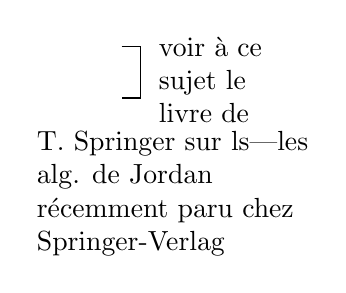
\begin{tikzpicture}[x=1cm,y=1cm]
\draw (0,2.15)--(.24,2.15)--(.24,1.5)--(0,1.5);
\node[anchor=north west,align=left] at (.35,2.4) {voir à ce\\sujet le\\livre de};
\node[anchor=north west,align=left] at (-1.2,1.2) {T. Springer sur \unsure{ls|les}\\alg. de Jordan\\récemment paru chez\\Springer-Verlag};
\end{tikzpicture}}}

\begin{center}\textsc{Séminaire}\end{center}

Le séminaire a continué celui de 1965/66, relatif aux \textit{groupes $p$-divisibles}. Il a comporté neuf exposés: quatre par Michel \textsc{Raynaud} et cinq par John \textsc{Tate} (qui en avait fait dix en 1965/66).

Michel \textsc{Raynaud} a rappelé les notions préliminaires nécessaires: schémas en groupes finis, dualité de Cartier, quotients. Il a ensuite donné la définition des groupes $p$-divisibles, et montré leur interprétation comme groupes formels. Dans son dernier exposé, il a démontré le théorème fondamental, dû à \textsc{Tate}, qui affirme que, en inégale caractéristique, le passage de l'anneau des entiers au corps des fractions définit un foncteur \textit{pleinement fidèle} sur la catégorie des groupes $p$-divisibles. Il est possible que sa démonstration, différente de celle de \textsc{Tate}, puisse être adaptée au cas d'égale caractéristique.

Les exposés de John \textsc{Tate} ont eu pour thème le \textit{théorème de relèvement} des variétés abéliennes, autrement dit le fait que relever une variété abélienne revient à relever le groupe $p$-divisible correspondant (la caractéristique résiduelle étant égale à $p$). A Woods Hole, en 1964, \textsc{Tate} en avait donné une démonstration basée sur une certaine construction cohomologique. Dans le séminaire, il a proposé une autre méthode, où variété abéliennes et groupes $p$-divisibles n'interviennent que par les \textit{faisceaux} correspondants (pour des topologies d'\textsc{Artin-Grothendieck} convenables). Cette méthode, malgré des difficultés techniques qui n'ont pas été entièrement résolues, paraît plus naturelle que la précédente, et de portée plus générale.

4
\margin{20}
